\documentclass[12pt]{article}

% Import images
\usepackage{graphicx}


\begin{document}
\title{PageRank}
\author{Vincent Foriel}

\maketitle
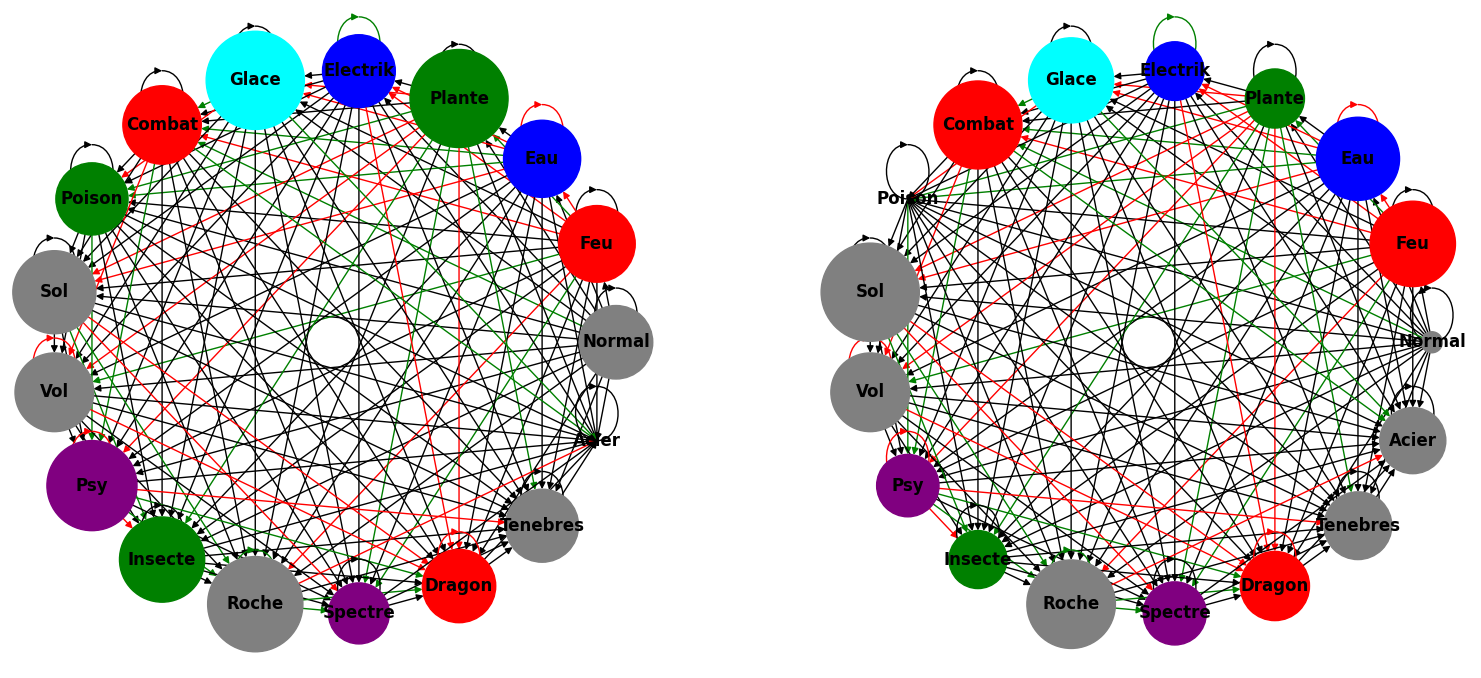
\includegraphics[width=\textwidth]{images/pokemon.png}
\newpage
\tableofcontents
\newpage

\section{Introduction}
The objective of this practical work is to study the PageRank algorithm by applying it in simple situations.

\begin{figure}[ht]
    \centering
    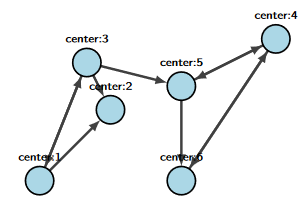
\includegraphics{images/graph.png}
    \caption{A simple oriented graph}
    \label{fig:graph}
\end{figure}

\section{The PageRank vector}

We consider the graph represented in Fig \ref{fig:graph}. In our exercise, each node represent a website, and each link represent a button or an hypertext link that redirect to another website. The objective is to determine the probability of being in each nodes after a huge number of steps (one step represent a redirection on another website)


For a random surfer that start his journey on a random node and with a dumping factor at 0.85, he have these chances to finish at each node:

\begin{center}
\begin{tabular}{c}
Node 1 : 0.0517050169447207\\
Node 2 : 0.0736797339206392\\
Node 3 : 0.0574127283822214\\
Node 4 : 0.3487031406768242\\
Node 5 : 0.1999036807831220\\
Node 6 : 0.2685956992924724  
\end{tabular}
\end{center}

This stability is reached after 23 steps.\\

\begin{figure}
    \centering
    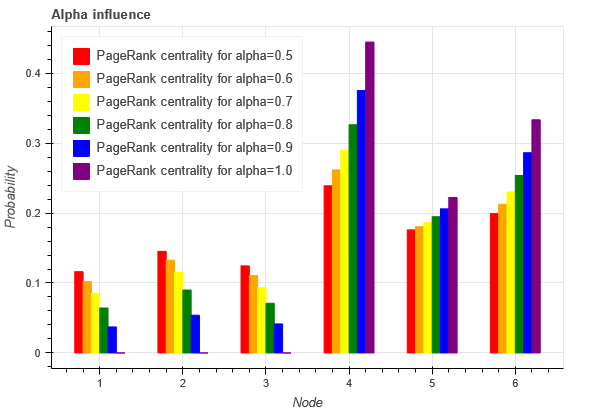
\includegraphics[width=\textwidth]{images/alpha.png}
    \caption{Influence of the dumping factor}
    \label{fig:alpha}
\end{figure}

Now, if we change the dumping factor and makes it increase from 0.5 to 1, we can see that the probability change i.e. Fig \ref{fig:alpha}. The greater the dumping factor is, the more chances the surfer has to leave the left part of the graph and stay on the right part.\

In comparison, degree centrality gives us:

\begin{center}
\begin{tabular}{c}
    Node 1 : 0.15\\
    Node 2 : 0.10\\
    Node 3 : 0.20\\
    Node 4 : 0.20\\
    Node 5 : 0.20\\
    Node 6 : 0.15
\end{tabular}
\end{center}

\begin{figure}[ht]
    \centering
    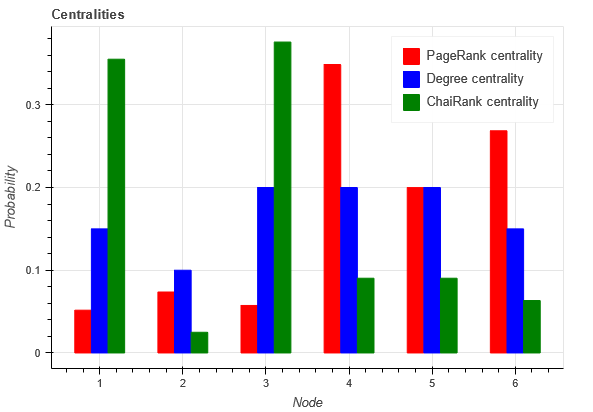
\includegraphics[width=\textwidth]{images/centralities.png}
    \caption{Centralities for the differents methods}
    \label{fig:centralitiesl}
\end{figure}

\section{The CheiRank vector}

For ChaiRank, with a dumping factor of 0.85, we got the following probabilites:

\begin{center}
\begin{tabular}{c}
Node 1 : 0.3550956514060691\\
Node 2 : 0.0250000000000000\\
Node 3 : 0.3758472962936703\\
Node 4 : 0.0903328050722020\\
Node 5 : 0.0903328050722020\\
Node 6 : 0.0633914421558570
\end{tabular}
\end{center}

This stability is reached after 68 steps.\\

\begin{figure}[ht]
    \centering
    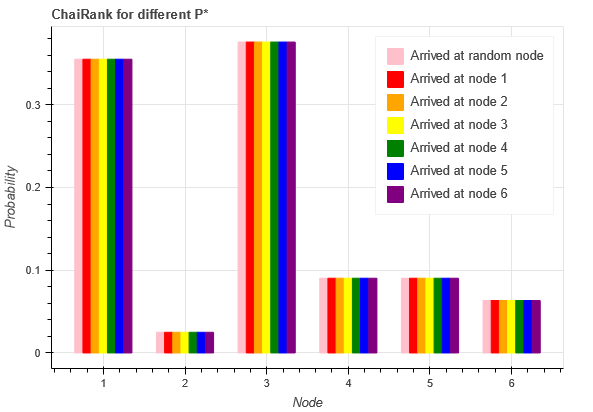
\includegraphics[width=\textwidth]{images/cheirank.png}
    \caption{Best referrers depending of the arrival website}
    \label{fig:cheirank}
\end{figure}

We can observe the difference between the 3 methods in the Fig \ref{fig:centralitiesl}. As we expected, the CheiRank vector seem to give more importance to the node that have the most outgoing links. My interpretation is that this vector can allow to create a referencing of biggest referrers.\\

By changing the arrival website, we can see on the Fig \ref{fig:cheirank} that the probabilities of the referring website are exactly the same. As the Fig \ref{fig:evolution} show, the CheiRank vector tends quickly to it's final state. We can draw the same graph with different starting node, we always see the same convergence values.

\begin{figure}[ht]
    \centering
    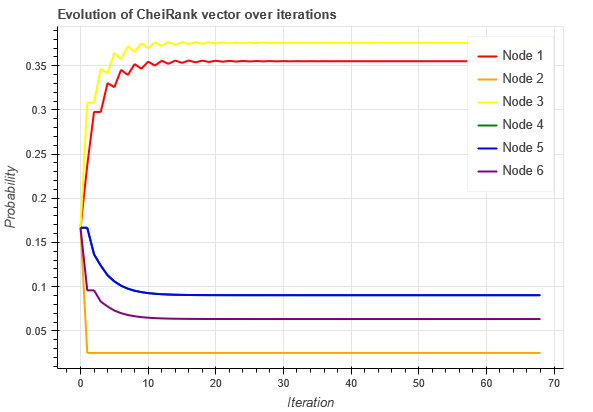
\includegraphics[width=\textwidth]{images/evolution.png}
    \caption{Evolution of the CheiRank vector}
    \label{fig:evolution}
\end{figure}


\section{PageRank : Pokémon, link them all!}

The adjency matric represent basically the links and there respective "strenght" between the different  network nodes. The stochastic matrix is more interested in the number of possible ways to leave/arrive from a given node.

\section{Conclusion}

For the first graph, the objective of the PageRank (resp. CheiRank) seems to be the ranking of the most referred (resp. referrer) websites. However, when we use them for a more complexe graph like the pokemon one, the interpretation becomes less evident.

At first sight, by looking the lines of the matrix, I noticed that the Pokemon that is the best ranked in the CheiRank vector seems to correspond to a Pokemon that have one of the greatest number of critical damages with not many unefficients attacks. I computed the ratio of attack and defense and I put the data in a table (in the data/analysis.ods file) to see the link between the rankings and these ratio. We can see that the CheiRank seems to correspond to the types that have the greatest damage ratio, and the PageRank seems to correspond to types that have the best defense ratio. Howerver, there is some little exceptions that I can't explain with this hypothesis.

\begin{figure}[ht]
    \centering
    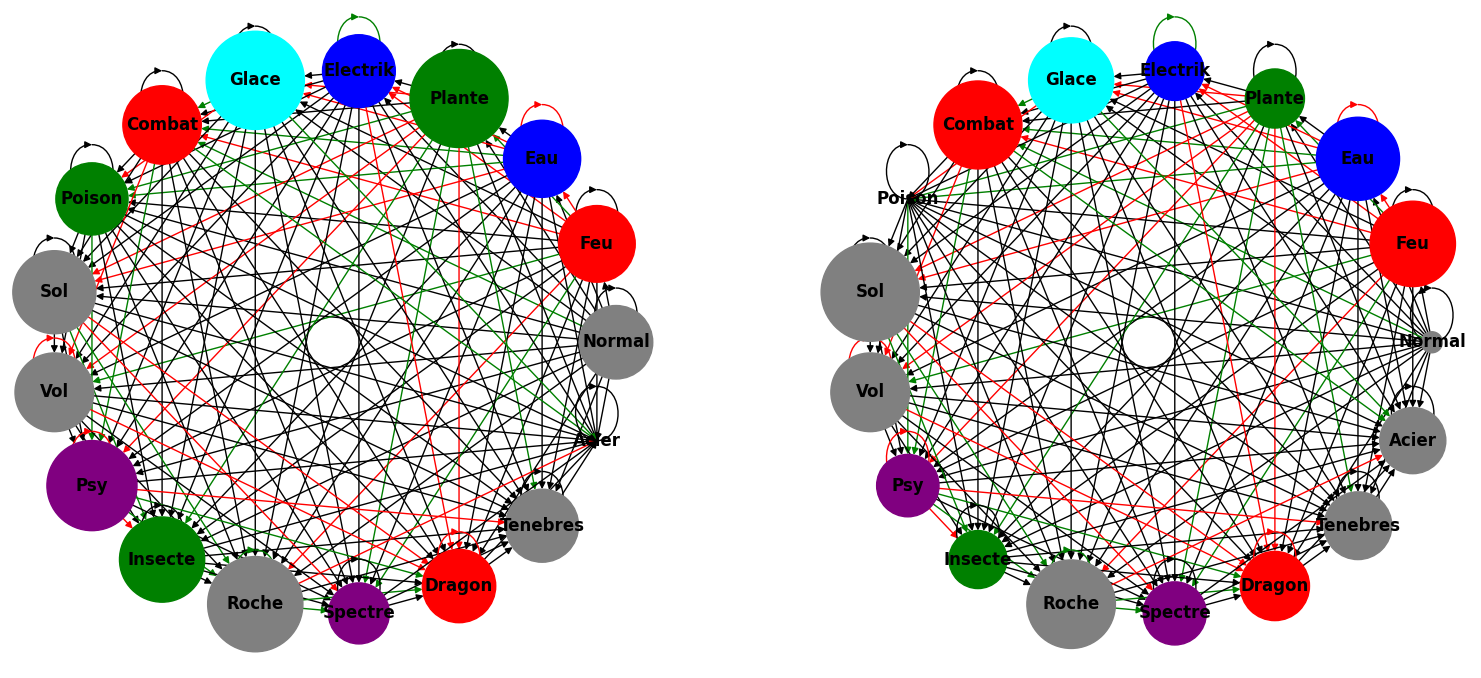
\includegraphics[width=\textwidth]{images/pokemon.png}
    \caption{Pokemon interactions and ranking with PageRank (left) and CheiRank (right)}
    \label{fig:pokemons}
\end{figure}

\begin{figure}[ht]
    \centering
    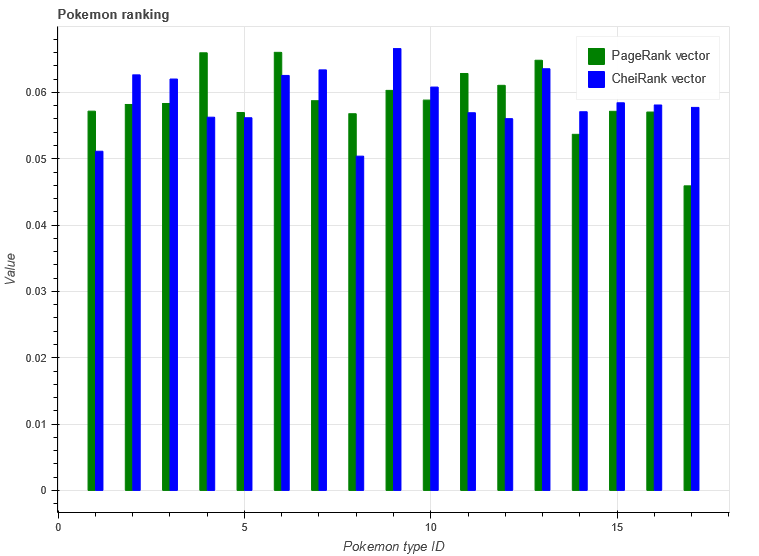
\includegraphics[width=\textwidth]{images/pokerank.png}
    \caption{Pokemon ranking}
    \label{fig:pokerank}
\end{figure}

\end{document}
